\section{Methodology}
\label{sec:methodology}

This section presents the proposed boundary-aware rationale selection method. The method is designed as an extension of rationale-based distillation: a teacher large language model first generates task labels and natural-language rationales, then a smaller student model is trained with label supervision and rationale supervision. Our contribution is inserted between rationale generation and student training. Instead of using all generated rationales directly, we select rationales that are more reliable and more suitable for student learning.

\begin{figure}[H]
    \centering
    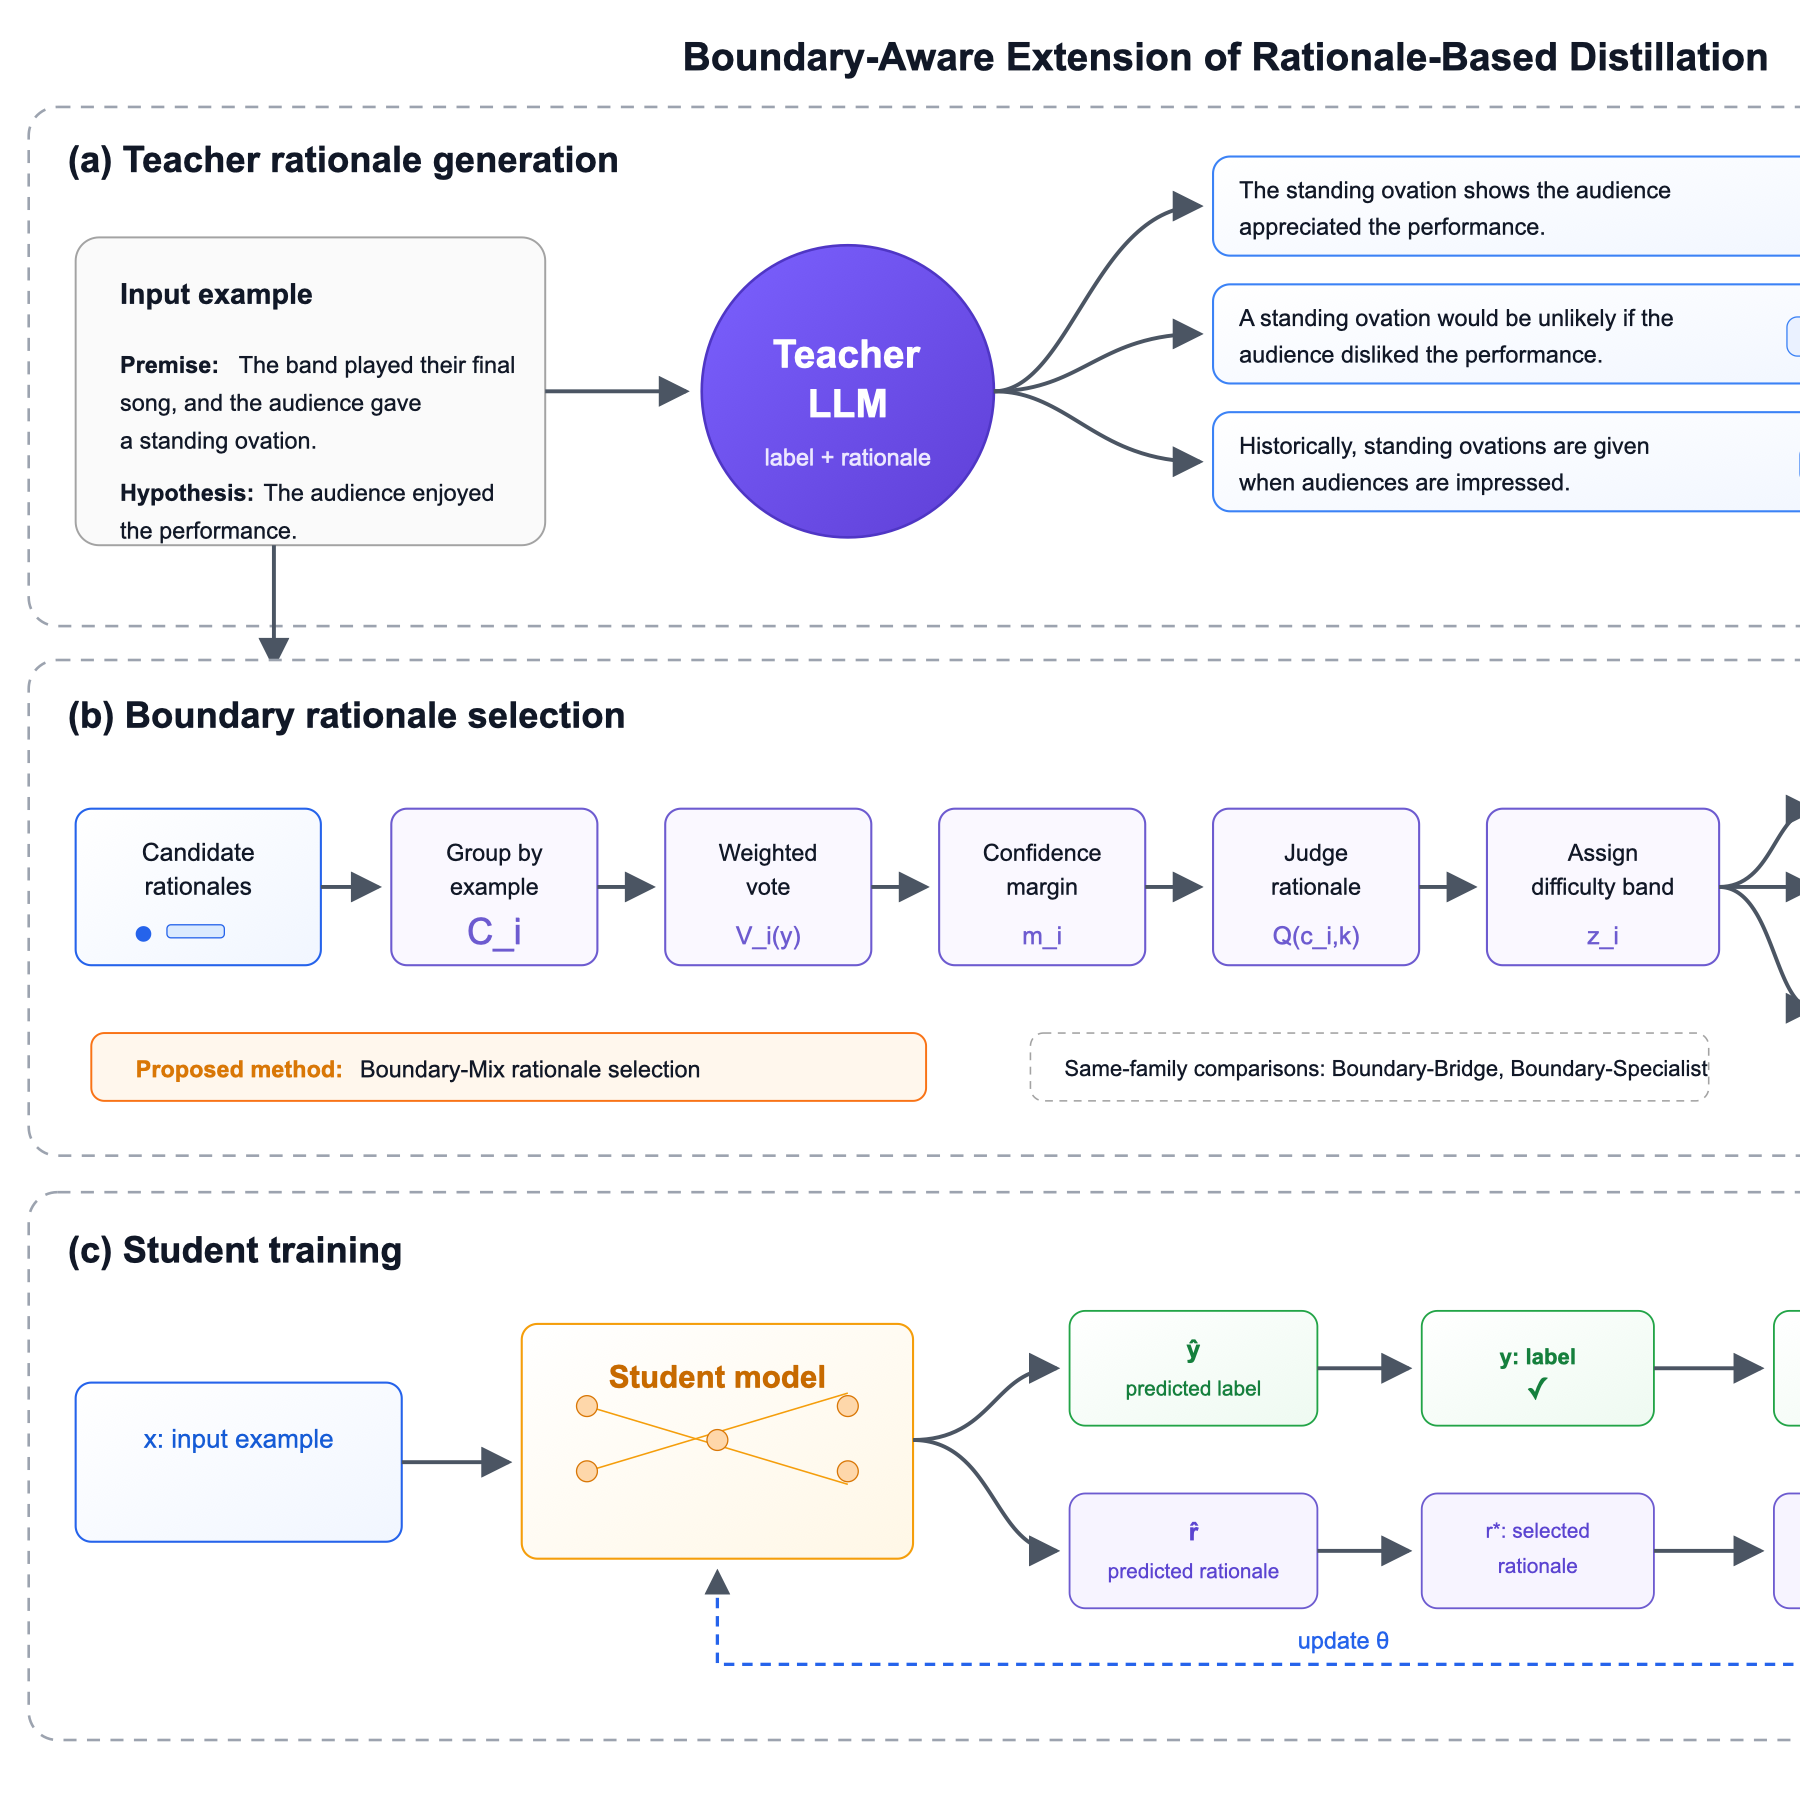
\includegraphics[width=\linewidth]{assets/boundary_methodology_academic_pipeline.png}
    \caption{Overall framework. Figure~\ref{fig:full-methodology}(a) shows teacher rationale generation. Figure~\ref{fig:full-methodology}(b) shows where the proposed boundary-aware rationale selection module is inserted. Figure~\ref{fig:full-methodology}(c) shows student training with selected rationales.}
    \label{fig:full-methodology}
\end{figure}

Figure~\ref{fig:full-methodology} shows the complete training framework. Figure~\ref{fig:full-methodology}(a) describes teacher rationale generation, Figure~\ref{fig:full-methodology}(b) shows where the boundary-aware module is inserted, and Figure~\ref{fig:full-methodology}(c) shows student training. Figure~\ref{fig:boundary-detail} expands the internal structure of the boundary-aware module. The proposed method does not change the teacher LLM, the student architecture, or the inference procedure. It changes the quality of the training supervision by filtering and selecting rationales before the student-training objective is applied.

\subsection{Teacher Rationale Generation}
\label{sec:teacher-generation}

Figure~\ref{fig:full-methodology}(a) represents the teacher rationale generation stage. For textual entailment, each input example is represented as
\begin{equation}
    x_i = (p_i, h_i), \quad y_i \in \mathcal{Y}.
    \label{eq:input-example}
\end{equation}

In Eq.~\eqref{eq:input-example}, $x_i$ is the $i$-th input example, $p_i$ is the premise, $h_i$ is the hypothesis, $y_i$ is the target task label, and $\mathcal{Y}$ is the complete label space. For textual entailment, $\mathcal{Y}$ contains labels such as entailment, contradiction, and neutral.

The teacher LLM is prompted to infer the relationship between the premise and hypothesis and to generate both a predicted label and a rationale. The teacher is asked to generate several rationale styles for the same example, including causal, contrastive, historical, conditional, neutral, consensus, and comparative rationales. The motivation is that different rationale styles expose different reasoning views of the same input. For each example, all generated rationales form a candidate set:
\begin{equation}
    C_i = \{c_{i,1}, c_{i,2}, \ldots, c_{i,K}\}.
    \label{eq:candidate-set}
\end{equation}

In Eq.~\eqref{eq:candidate-set}, $C_i$ is the candidate set for example $x_i$, $K$ is the number of generated rationale candidates for that example, and $c_{i,k}$ is the $k$-th candidate. Each candidate is defined as
\begin{equation}
    c_{i,k} = (r_{i,k}, \hat{y}_{i,k}, s_{i,k}).
    \label{eq:candidate-tuple}
\end{equation}

In Eq.~\eqref{eq:candidate-tuple}, $r_{i,k}$ is the generated rationale, $\hat{y}_{i,k}$ is the label predicted with that rationale, and $s_{i,k}$ is the rationale source or rationale type. At this stage, generated rationales are not treated as final training targets. They are treated as candidates that must pass the boundary-aware selection stage before being used for student supervision.

\subsection{Boundary-Aware Rationale Selection}
\label{sec:boundary-selection}

Figure~\ref{fig:full-methodology}(b) marks the proposed boundary-aware rationale selection stage in the full framework, and Figure~\ref{fig:boundary-detail} gives the detailed view of this module. The purpose of this stage is to transform a noisy pool of generated rationales into a smaller set of rationales that are more suitable for student learning. The module follows three levels: a shared rationale selection pipeline in Figure~\ref{fig:boundary-detail}(a), a difficulty-band assignment step in Figure~\ref{fig:boundary-detail}(b), and same-family selection variants in Figure~\ref{fig:boundary-detail}(c).

\begin{figure}[H]
    \centering
    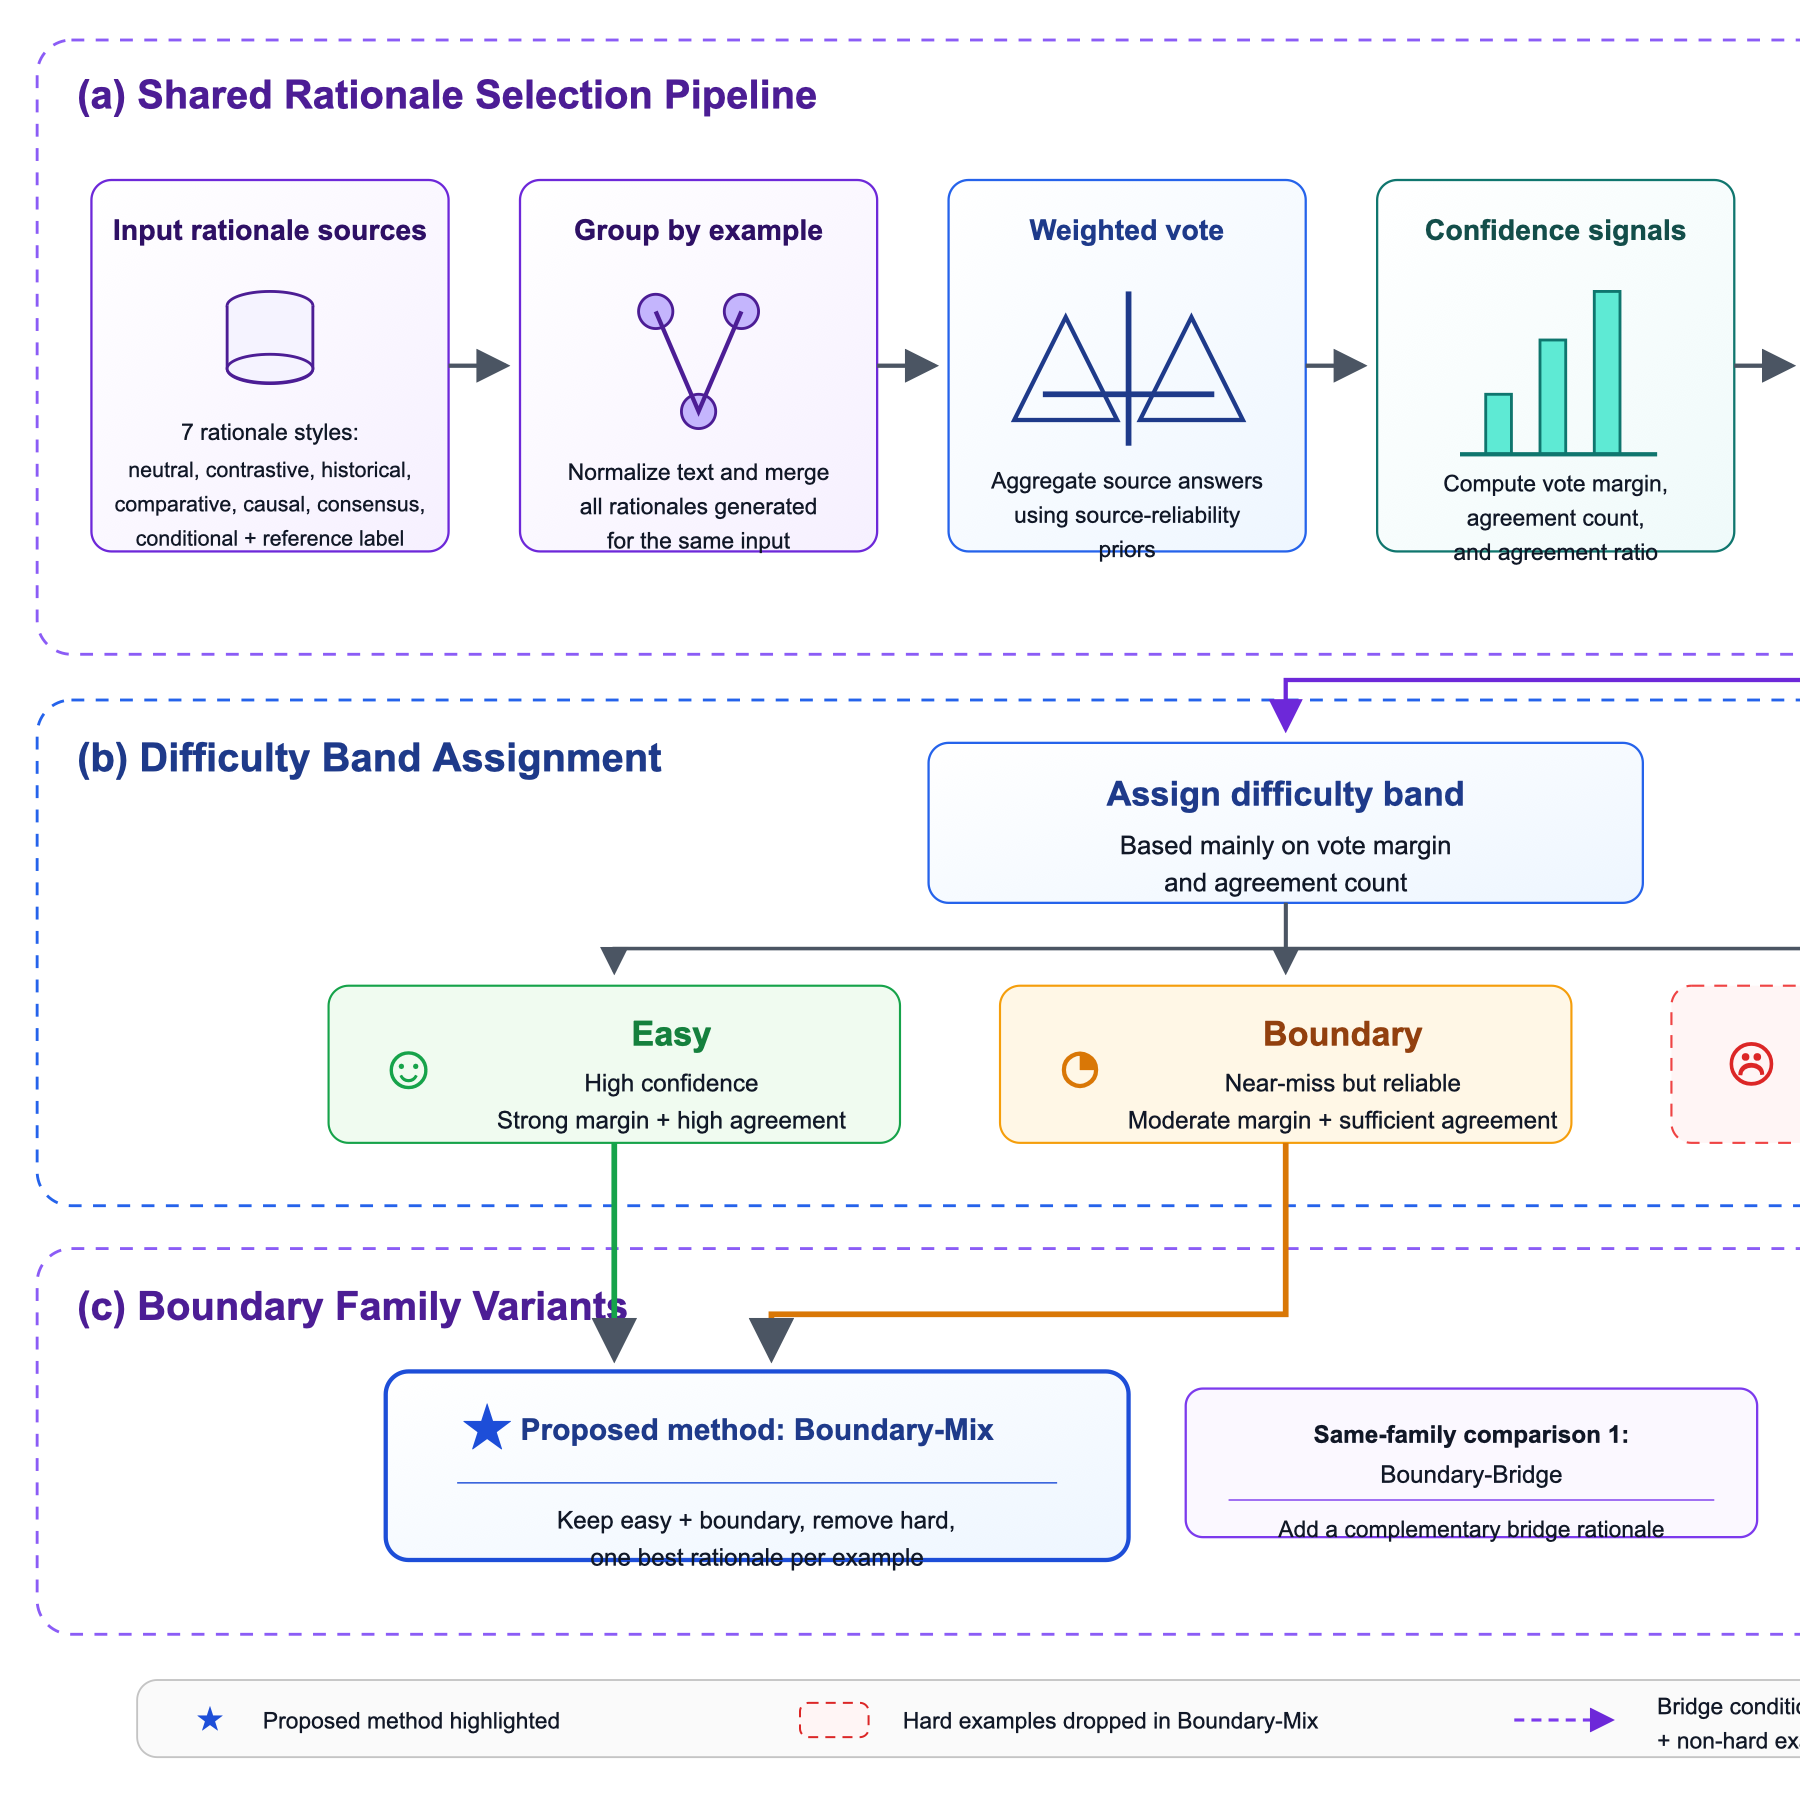
\includegraphics[width=\linewidth]{assets/boundary_selection_detail_pipeline.png}
    \caption{Detailed boundary-aware rationale selection module. Figure~\ref{fig:boundary-detail}(a) shows the shared rationale selection pipeline. Figure~\ref{fig:boundary-detail}(b) assigns examples into easy, boundary, and hard bands. Figure~\ref{fig:boundary-detail}(c) summarizes Boundary-Mix and the same-family comparison variants.}
    \label{fig:boundary-detail}
\end{figure}

The first step is grouping. Candidate rationales are normalized and grouped by the same original input $x_i$, so all rationales generated for the same premise-hypothesis pair are compared together. The second step is weighted label voting. For each possible label $y$, the method sums the contribution of candidates that predict that label:
\begin{equation}
    V_i(y) = \sum_{k=1}^{K} w(s_{i,k}) \cdot \mathbf{1}[\hat{y}_{i,k} = y].
    \label{eq:weighted-vote}
\end{equation}

In Eq.~\eqref{eq:weighted-vote}, $V_i(y)$ is the vote score for label $y$ on example $x_i$, $w(s_{i,k})$ is the reliability weight of source $s_{i,k}$, and $\mathbf{1}[\cdot]$ is an indicator function that returns 1 when candidate $k$ predicts label $y$ and 0 otherwise. The source weight is a source-reliability prior over rationale styles. It controls how strongly each rationale source contributes to the vote.

The voted label is selected by
\begin{equation}
    \hat{y}^{vote}_i = \arg\max_{y \in \mathcal{Y}} V_i(y).
    \label{eq:voted-label}
\end{equation}

In Eq.~\eqref{eq:voted-label}, $\hat{y}^{vote}_i$ is the group-level voted label for example $x_i$. It is the label with the highest weighted vote among all labels in $\mathcal{Y}$.

Confidence is measured by several signals. The main signal is the vote margin, defined as the distance between the strongest label vote and the second strongest label vote:
\begin{equation}
    m_i = V_i(\hat{y}^{vote}_i) -
    \max_{y \ne \hat{y}^{vote}_i} V_i(y).
    \label{eq:vote-margin}
\end{equation}

In Eq.~\eqref{eq:vote-margin}, $m_i$ is the vote margin. The first term is the vote score of the winning label, and the second term is the strongest competing label score. A larger margin means stronger label agreement.

We also compute agreement count and agreement ratio:
\begin{equation}
    a_i = \sum_{k=1}^{K} \mathbf{1}[\hat{y}_{i,k} = \hat{y}^{vote}_i],
    \quad
    \rho_i = \frac{a_i}{K}.
    \label{eq:agreement}
\end{equation}

In Eq.~\eqref{eq:agreement}, $a_i$ is the number of candidates that support the voted label, and $\rho_i$ is the fraction of candidates that support the voted label.

These signals define the difficulty band:
\begin{equation}
    z_i =
    \begin{cases}
        \text{easy}, & m_i \ge \tau_m^{easy} \land \rho_i \ge \tau_\rho^{easy}, \\
        \text{boundary}, & m_i \ge \tau_m^{boundary} \land a_i \ge \tau_a^{boundary}, \\
        \text{hard}, & \text{otherwise}.
    \end{cases}
    \label{eq:difficulty-band}
\end{equation}

In Eq.~\eqref{eq:difficulty-band}, $z_i$ is the assigned difficulty band. $\tau_m^{easy}$ and $\tau_\rho^{easy}$ are thresholds for easy examples. $\tau_m^{boundary}$ and $\tau_a^{boundary}$ are minimum thresholds for retaining boundary examples. Examples that fail these conditions are treated as hard. Easy examples have strong margin and high agreement. Boundary examples are near-miss cases with moderate confidence but sufficient agreement. Hard examples have low confidence or noisy agreement and are dropped by Boundary-Mix.

After assigning the difficulty band, the method judges each rationale candidate. A useful rationale should support the voted label, be grounded in the premise and hypothesis, explicitly connect the reasoning to the answer, and have an appropriate length for supervision. We combine these signals into a rationale quality score:
\begin{equation}
\begin{aligned}
    Q(c_{i,k}) =
    &\alpha S_{label}(c_{i,k})
    + \beta S_{ground}(c_{i,k})
    + \gamma S_{answer}(c_{i,k}) \\
    &+ \delta S_{source}(c_{i,k})
    + \eta S_{brief}(c_{i,k}).
\end{aligned}
    \label{eq:rationale-quality}
\end{equation}

In Eq.~\eqref{eq:rationale-quality}, $Q(c_{i,k})$ is the quality score of candidate $c_{i,k}$. $S_{label}$ checks whether the candidate label agrees with the voted label. $S_{ground}$ checks whether the rationale is connected to the premise and hypothesis instead of introducing unsupported information. $S_{answer}$ checks whether the rationale explicitly supports the final answer. $S_{source}$ incorporates the rationale-type prior, and $S_{brief}$ penalizes rationales that are too weak or too verbose for effective supervision. The coefficients $\alpha$, $\beta$, $\gamma$, $\delta$, and $\eta$ control the contribution of each scoring signal.

The source-prior term is defined as a label-source compatibility lookup:
\begin{equation}
    S_{source}(c_{i,k}) =
    \operatorname{Prior}(y_i, s_k),
    \label{eq:source-score}
\end{equation}
where $y_i$ is the selected training label for example $i$, and $s_k$ is the rationale source type of candidate $c_{i,k}$. The prior itself is:
\begin{equation}
    \operatorname{Prior}(y, s) =
    \begin{cases}
        P_{y,s}, & \text{if } (y,s) \in \mathcal{Y} \times \mathcal{S}, \\
        0, & \text{otherwise}.
    \end{cases}
    \label{eq:source-prior}
\end{equation}
Here, $P \in [0,1]^{|\mathcal{Y}| \times |\mathcal{S}|}$ is a manually specified compatibility matrix between task labels and rationale source types. The value is not learned from model training and is not a direct copy of original-paper performance. Instead, it encodes the expected relationship between each rationale type and each label. For example, comparative and contrastive rationales are expected to be more useful for contradiction because they highlight differences or conflicts, while if--else rationales are expected to be more useful for neutral because they often express uncertainty or conditional reasoning.

\begin{table}[H]
\centering
\caption{Source-prior compatibility matrix $P_{y,s}$ used for boundary-aware rationale scoring.}
\label{tab:source-prior-matrix}
\begin{tabular}{p{0.18\linewidth} r r r r r r r}
\hline
Label $y$ & causal & neutral & contrastive & historical & comparative & consensus & if--else \\
\hline
entailment & 0.92 & 0.88 & 0.95 & 1.00 & 0.70 & 0.98 & 0.74 \\
neutral & 0.84 & 0.96 & 0.90 & 0.72 & 0.99 & 0.82 & 1.00 \\
contradiction & 0.97 & 0.89 & 0.99 & 0.74 & 1.00 & 0.84 & 0.70 \\
\hline
\end{tabular}
\end{table}

The same prior is also used during weighted voting. If candidate $c_{i,k}$ predicts label $\hat{y}_{i,k}$ and comes from source $s_k$, then the weighted vote score for label $y$ is:
\begin{equation}
    V_i(y) =
    \sum_{k=1}^{K_i}
    \mathbb{1}[\hat{y}_{i,k}=y]
    \operatorname{Prior}(y, s_k).
    \label{eq:weighted-vote-prior}
\end{equation}
Thus, a candidate contributes more strongly when its rationale source is compatible with the label it predicts. This makes the voting and rationale-scoring stages consistent: both prefer candidate labels and rationales whose source type matches the expected reasoning pattern for the selected label.

\subsection{Boundary-Mix and Same-Family Variants}
\label{sec:boundary-variants}

Figure~\ref{fig:boundary-detail}(c) summarizes the boundary-family variants. The main proposed method is Boundary-Mix. It follows the full selection process in Figure~\ref{fig:boundary-detail}(a) and Figure~\ref{fig:boundary-detail}(b): candidate rationale collection, grouping by example, weighted vote, confidence signal estimation, rationale judging, difficulty-band assignment, and final selection. Boundary-Mix keeps examples in the easy and boundary regions because they contain usable supervision. It removes hard examples because their generated rationales are too unstable.

Formally, Boundary-Mix selects the highest-scoring rationale for examples that are not hard:
\begin{equation}
    c_i^* =
    \arg\max_{c_{i,k} \in C_i} Q(c_{i,k}),
    \quad \text{if } z_i \in \{\text{easy}, \text{boundary}\}.
    \label{eq:boundary-mix-selection}
\end{equation}

In Eq.~\eqref{eq:boundary-mix-selection}, $c_i^*$ is the selected rationale candidate for example $x_i$. It is the candidate with the highest quality score among candidates in $C_i$, but only when the example is assigned to the easy or boundary band. If $z_i = \text{hard}$, then $x_i$ is removed from rationale-supervised training.

\begin{table}[H]
\centering
\caption{Boundary family variants.}
\label{tab:boundary-family-variants}
\begin{tabular}{p{0.18\linewidth} p{0.40\linewidth} p{0.32\linewidth}}
\hline
Variant & Selection rule & Purpose \\
\hline
Boundary-Mix &
Selects the highest-scoring rationale from easy and boundary examples; removes hard examples. &
Main proposed method. It balances rationale quality and training coverage. \\
\hline
Boundary-Bridge &
Selects the main rationale and optionally adds a second complementary rationale with a different reasoning view. &
Tests whether adding one diverse rationale improves learning beyond single-rationale selection. \\
\hline
Boundary-Specialist &
Uses the same boundary pipeline but emphasizes stronger rationale sources or rationale types. &
Supports analysis of source reliability and label-rationale compatibility. \\
\hline
\end{tabular}
\end{table}

The same-family variants are useful for controlled comparison. Boundary-Bridge studies whether adding one complementary rationale can improve training. Boundary-Specialist studies whether stronger rationale sources or rationale types should be emphasized. Because these variants share the same upstream boundary pipeline, their comparison helps isolate the effect of the final selection rule.

\subsection{Student Training with Selected Rationales}
\label{sec:student-training}

Figure~\ref{fig:full-methodology}(c) shows the student training stage. The student model is trained in a text-to-text framework, where the same input $x_i$ can be paired with different task prefixes. With the label prefix, the model learns to generate the task label. With the rationale prefix, the model learns to generate the selected rationale. This makes rationale learning an auxiliary task instead of an additional inference-time input.

The label prediction loss is defined as the average cross-entropy between the student prediction and the target label:
\begin{equation}
    \mathcal{L}_{label}
    = \frac{1}{N}\sum_{i=1}^{N}
    \ell(f_\theta(x_i, [label]), y_i).
    \label{eq:label-loss}
\end{equation}

In Eq.~\eqref{eq:label-loss}, $N$ is the number of training examples, $f_\theta$ is the student model with parameters $\theta$, $[label]$ is the task prefix that asks the model to generate the label, and $\ell$ is token-level cross-entropy loss.

The rationale generation loss is computed in the same way, but the target is the selected rationale $r_i^*$ produced by the boundary-aware selection stage:
\begin{equation}
    \mathcal{L}_{rationale}
    = \frac{1}{N}\sum_{i=1}^{N}
    \ell(f_\theta(x_i, [rationale]), r_i^*).
    \label{eq:rationale-loss}
\end{equation}

In Eq.~\eqref{eq:rationale-loss}, $[rationale]$ is the rationale prefix that asks the student to generate a rationale, and $r_i^*$ is the selected rationale from Boundary-Mix.

The complete multi-task objective balances the two losses:
\begin{equation}
    \mathcal{L}
    = \lambda \mathcal{L}_{label}
    + (1-\lambda)\mathcal{L}_{rationale}.
    \label{eq:multitask-loss}
\end{equation}

In Eq.~\eqref{eq:multitask-loss}, $\lambda$ controls the trade-off between label prediction and rationale generation. When $\lambda$ is larger, training emphasizes label prediction; when it is smaller, training gives more weight to rationale generation.

This training setup preserves the deployment advantage of rationale-based distillation. During inference, the teacher LLM, candidate rationales, and boundary selector are not used. The trained student receives only the input example and predicts the task label directly. Therefore, the boundary-aware module improves the training data while keeping the student architecture and inference process unchanged.
